\documentclass[11pt]{article}
\usepackage{graphicx}
\usepackage{caption}
\usepackage{chngcntr}
\usepackage[section]{placeins} % subsections
\usepackage[round, sort, numbers]{natbib}
\usepackage{makecell}
\usepackage{url}
\counterwithin{figure}{section}
\captionsetup[figure]{slc=off}
\usepackage[left=2cm, right=2cm, top=2cm, bottom=2cm]{geometry} % geometry of page
\setcitestyle{square} % square referencing style
\usepackage[fleqn]{amsmath} % for maths
\usepackage{subfig}
\setlength{\parindent}{0pt} % no indents on new paragraphs
\graphicspath{{Code/Analysis/Figures/}}

\newcommand*\ruleline[1]{\par\noindent\raisebox{.8ex}{\makebox[\linewidth]{\hrulefill\hspace{1ex}\raisebox{-.8ex}{#1}\hspace{1ex}\hrulefill}}}

\begin{document}
\begin{titlepage}

    \begin{center}
        \vspace*{1cm}
        \Huge
        \textbf{Robotics} \\
        \vspace{0.5cm}
        \LARGE
        \vspace{1.5cm}
        \textbf{G. Sheppard, D. Thomas, J. Doering, J. Matthews, C. Li} \\
        \vfill
        \vspace{0.8cm}
        \Large
        University of Birmingham\\
        Physics and Astronomy Department\\
    \end{center}
\end{titlepage}

\tableofcontents

\section{Abstract}
Wow look at \ref{angleplot}. \cite{Bae2006}.

\section{Introduction}
\subsection{Background}
\subsection{Motivation}
\subsection{Theory}

\section{Connecting}
\subsection{Nao}


David: you know what to write
also David write about how you sped up NAO's kicks somewhere it's juicy and tasty info/
Connecting to NAO: 

Include diagram of joints and talk about connecting and extracting sensor values and calling joints using python dictionaries:
Normalising speeds, creating algorithms to ensure simultaneity.
Slowing initial speed of NAO to prevent injury during initialisation of positions.
Defining positions to ensure left and right side was symmetric and improved on previous years positions my maximising the range of motion with fail safes to ensure a correct position was reached by comparing joint data with expected position\\

Small amount about compatibility issues and that these were resolved by using the same python SDK and choreagraph versions and running code via linux to prevent issues with compiling and installing : limit section to 100 words.


\subsection{Hinge Encoders}
\ruleline{George Sheppard}
There are two sets of hinge encoders used, the large/big encoder, and the small encoders. The large encoder record the angle from the vertical to the largest rod of the swing. The small encoders record the angle with respect to the previous rod, there are 2 on each side of the swing.\\

A large amount of time was invested into connecting to these hinge encoders from any computer other than the lab one. Unfortunately, due to the nature of the shared object files required by the encoders, the set up is complicated and it is advised to use the lab computer when using the hinge encoders.\\

A guide for setting up the hinge encoders is provided in the wiki found in \ref{sec:wiki}.


\section{Creating Algorithms}

\ruleline{George Sheppard}
\subsection{The Interface}
The creation of each individual algorithm required the use of a substantial amount of common code, such as the logic required for: connecting to Nao, collecting values from the hinge encoders and Nao, handling of previous collected values, switching Nao's position, and storage. For this reason an interface was created that functioned as a base that all algorithms were built off, the logic of this base code is illustrated in figure \ref{InterfaceLogic}. The interface starts by collecting all values required for the algorithm decision making process, it then passes these values through the algorithm, depending on the output of the algorithm it will either change Nao's position, switch to the next algorithm, or finish and store the data. It also fixes the sample rate to a specified frequency.\\

    \begin{figure}[!htb]
        \centering
        \captionbox
             {The logic behind the interface, all that required changing was the algorithm logic that the decision making was based on.\label{InterfaceLogic}}
             {\includegraphics[width=1.0\textwidth]{InterfaceLogic.eps}}
    \end{figure}

With this base structure in place, creating an algorithm involved one function that took a set of values, and decided how to react to them, the algorithm had access to all past data to help in decision making. As these algorithms were defined in the same way, it is easy to switch between different algorithms mid swing, such that the motion of NAO could be more stringently controlled. For example NAO could be told to increase to $30^o$, then maintain this amplitude for $10s$, and then finally decrease back down to $0^o$.\\

With this base structure in place, creating an algorithm had two requirements: it took the set of values given to it by the interface, and it returned either 'switch', None, or any of the named positions that were defined in the Robot subsection of the interface e.g. 'Seated', 'Extended' etc.\\

As the interface required the encoders and the robot to connect to, a series of mock classes were created that aimed to replicate their functionality. This meant that away from the lab these fake classes were used as a substitute such that the interface could be developed.

\subsection{Testing}
One of the advantages of this setup was the ability to test algorithms without connecting to either the robot or the hinge encoders. As all previous data collected in the lab were stored, a setup was developed that read the file in line by line and passed it through the algorithm. The results of this test were then stored to a file in the same way as normal, and as such data such as the kicking times of Nao could be plotted instantly.\\

One downside of this method was that the data being fed into the algorithm wasn't reactive to the previous decision of the algorithm, as all the data was pre-recorded. This meant that this method was in no way a replacement for testing the algorithm in the lab, but instead was used as a way to check that the algorithm is logically correct before spending time with Nao on it.


\section{Simple Pendulum}
\subsection{Start Up}

\ruleline{James Doering}

\textit{James: talk about two positions defined for the motion, idea behind the algorithm, how it links into the next algorithm that increases amplitude, results, why is it tricky to start off like this (have to predict when to swing very well sort of stuff), if multiple algorithms created do for each} \\

There are multiple tactics for beginning a swing from rest - the most intuitive is to "kick off" from an object to give an initial amplitude, which a human would achieve by pushing themselves from the floor. This method was approached by previous years by creating a box for the robot to push away, or by manually giving it an intial amplitude. This was further developed upon by giving the robot a method of starting with zero assistance. By utilising the angular velocity gained by the swing when the robot's legs swing (as described in section INSERT REF). \\

For the start-up algorithm, very little input is required - the motion is effectively pre-calculated, as the initial conditions are the same each time, with NAO starting from rest. Parametric motion cannot be used to start the swing, and so changes in angular momentum of NAO's legs must be used instead. To achieve this, two postures were defined: 'seated', with the legs tucked beneath the seat and the chest pulled in to the bar, and 'extended', with the legs extended out and the chest pushed away from the bar. These two postures can be seen in figure \ref{fig:seatedextended}.\\

    \begin{figure}
        \centering
        \includegraphics{}
        \caption{The 'seated' and 'extended' positions used in the start-up script and TORQUE method.}
        \label{fig:seatedextended}
    \end{figure}

The algorithm is very simple - an initial kick is made, going from the seated to the extended posture, which in turn gives the swing some small angular momentum. The robot does not move until a quarter-period has passes, when it should be at the peak of its backward swing. It then kicks into the seated position, and waits for a half period so it is at its next peak, before switching postures again. This loop of waiting a half-period and kicking is repeated until a minimum amplitude is reached (1 degree), where it then switches to another algorithm. This was done smoothly by only switching after a short time had passed since its last kick, preventing the next algorithm from immediately calling for a new kick.\\

This start-up was made even more effective by adding extra weight to the robot's feet, and so increasing the angular momentum produced in the swing - the difference in motion of the two methods can be seen in figure \ref{fig:startupcomparison}. This helped counteract the large mass of the swing and the small mass of NAO.


    \begin{figure}
        \centering
        \includegraphics[width=0.6\textwidth]{}
        \caption{A plot showing the difference in amplitude gained for the start-up script with the default robot and the robot with extra weight in its feet.}
        \label{fig:startupcomparison}
    \end{figure}



\subsection{Determining when to swing}
\ruleline{George Sheppard}
To create algorithms that are efficient at applying Nao's energy into the motion of the swing requires an accurate estimate of the maximum angle of the swing, or the time at which this occurs. To early a swing dissipates the energy, and too late doesn't take advantage of the boost in velocity caused by changing position.\\
For this reason a discussion of the best method for determining the maximum of the swing is outlined below.




\subsubsection{Angular Velocity}
\ruleline{Chenglong Li}
The angular Velocity algorithms uses the fact that the sign of the angular velocity will change just after the Nao hits its maxima. Therefore one can instruct the Nao to change its posture whenever the angular velocity change its sign. This algorithm is very easy to implement and very reliable. However, there are two serious weakness for this algorithm.The first one is that this algorithm do not learn from old data, which means that it will not keep improving itself. Before talking about the second weakness, one should understand the concept of 'offset' for the algorithm. Assuming the algorithm predicts Nao should change its posture at time T or angle A and one would like it to start change its position a little bit earlier before  

\subsubsection{Calculation of Max Angle}
Chenglong: Same as above

\subsubsection{Quarter Period}
\ruleline{George Sheppard}
The quarter period algorithm uses the time that the last quarter period of the cycle took to predict the time of the next maximum, and utilizes the fact that Nao's motion only increases in angle by a small amount per cycle. Whenever Nao swings through the first thing to calculate is an estimate of the time that Nao actually crossed the boundary. This is important as Nao swings the fastest through the centre, and therefore the first time recorded after he crossed may not be close enough to the true time. Shown in figure \ref{InterpolationDiagram} is a diagram of this situation. 

    \begin{figure}[!htb]
        \centering
        \captionbox
             {Illustration of the values of the swing, before and after the crossing point.\label{InterpolationDiagram}}
             {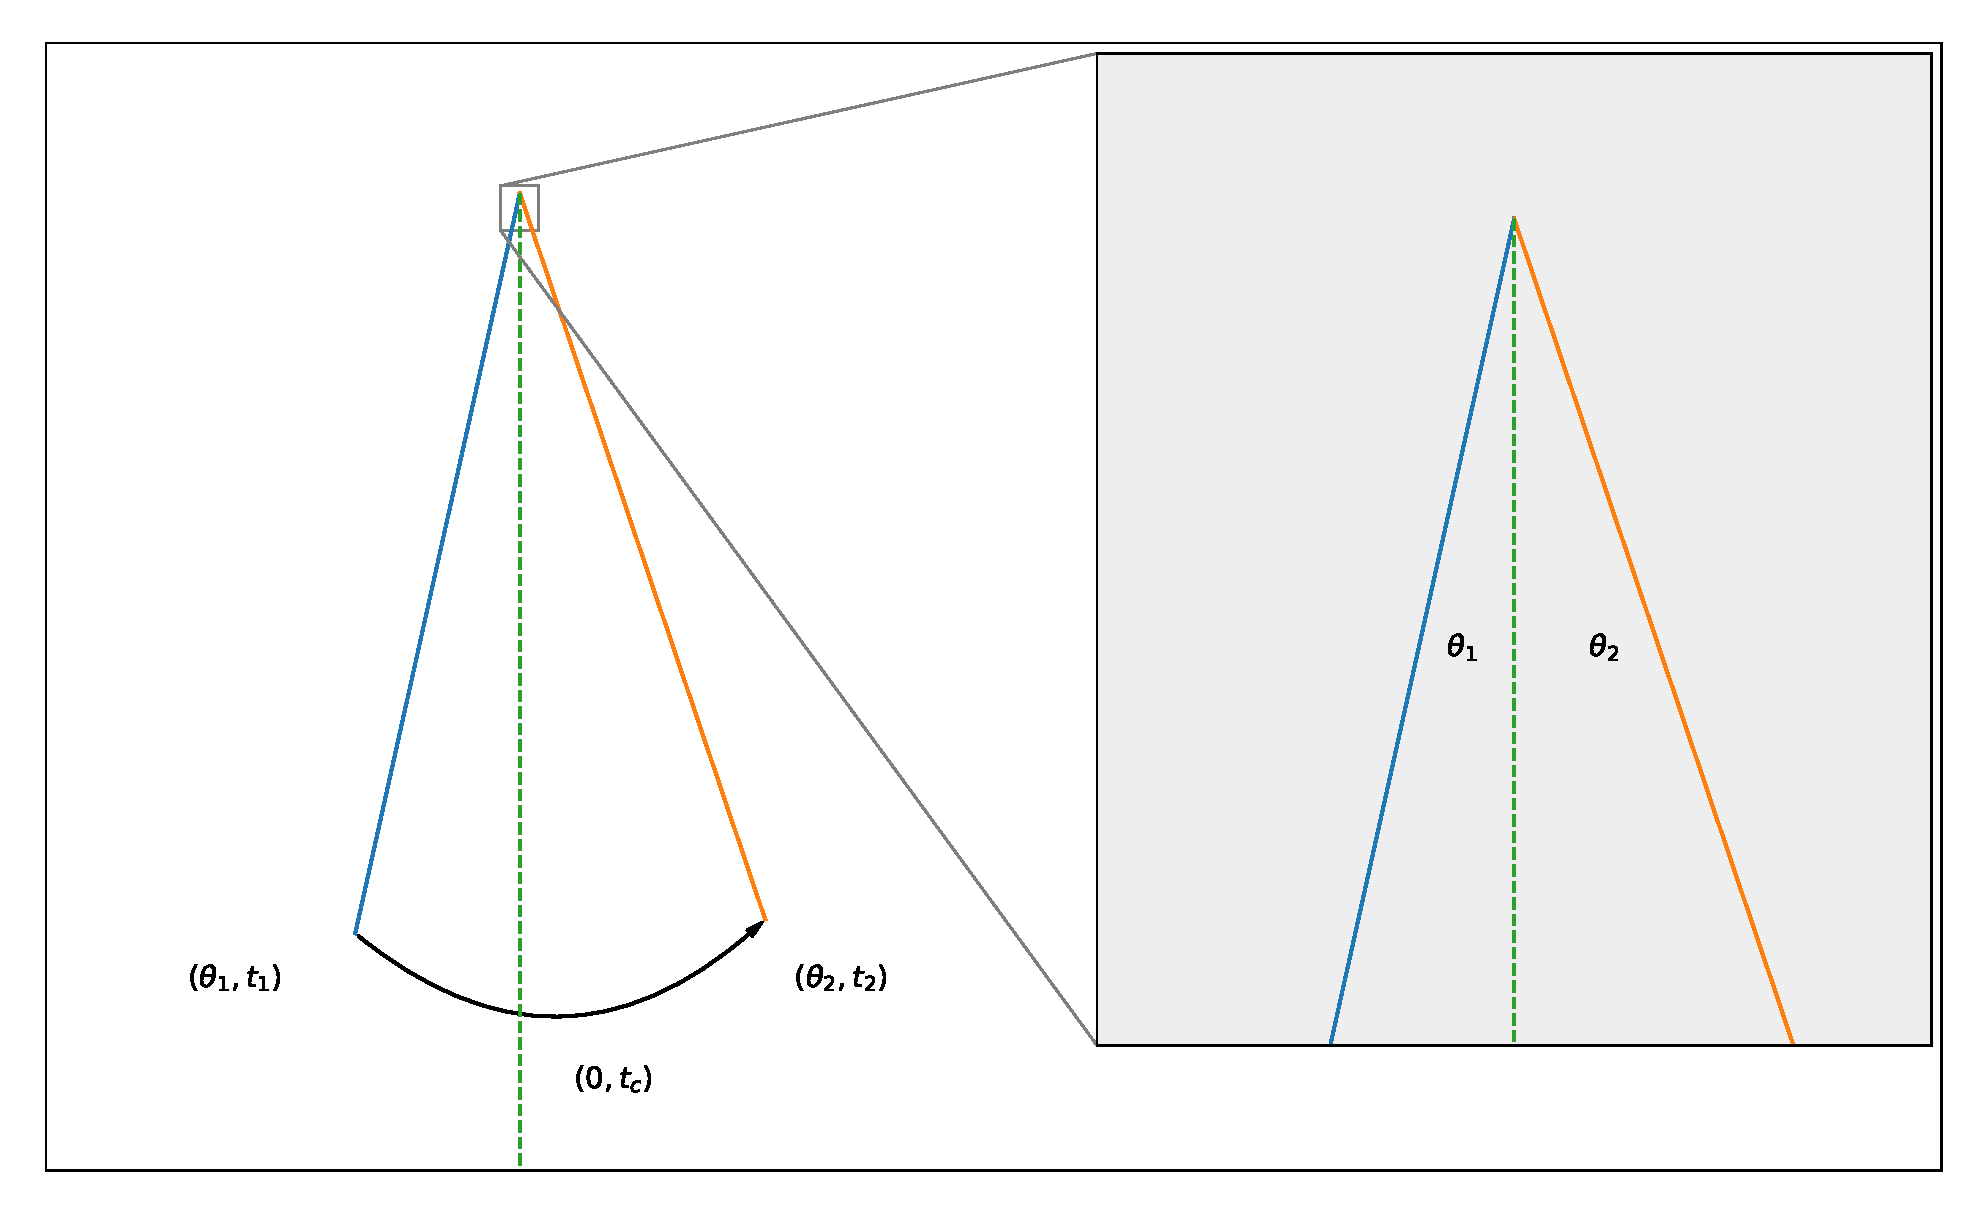
\includegraphics[width=1.0\textwidth]{InterpolationDiagram.eps}}
    \end{figure}

For angle and time $(\theta_1, t_1)$ before the crossing, and $(\theta_2, t_2)$ after the crossing, a linear interpolation can be applied to give a more accurate estimate of the true zero point crossing. This is calculated using

\begin{equation}
    t_c = t_2 - (t_2 - t_1) \frac{|\theta_2|}{|\theta_2 - \theta_1|}.
\end{equation}

As is expected for a higher sampling time this error on the true centre time is smaller. The second value to calculate is the time at which Nao was at the last angle maxima. This can be done simply as all previous values of the encoder are recorded. One small complication is the introduction of local maximas, these occur more often at low amplitude swings due to the jolted motion of Nao's movement, and need to be filtered out to allow a better estimate for the maximum angle time. To filter these local maxima out the moving average of the encoder values is calculated, this smooths the data, figure \ref{MovingAverageDiagram} shows a comparison between the moving average of some example data, for this example the latest local maximum would be the calculated max time, but after using the moving average the estimate is much closer to it's true point. Using the modified encoder values the time of the maximum can be determined, and therefore the quarter period of the swing can be calculated. \\

    \begin{figure}[!htb]
        \centering
        \captionbox
             {Comparison of angle data before and after a moving average is applied.\label{MovingAverageDiagram}}
             {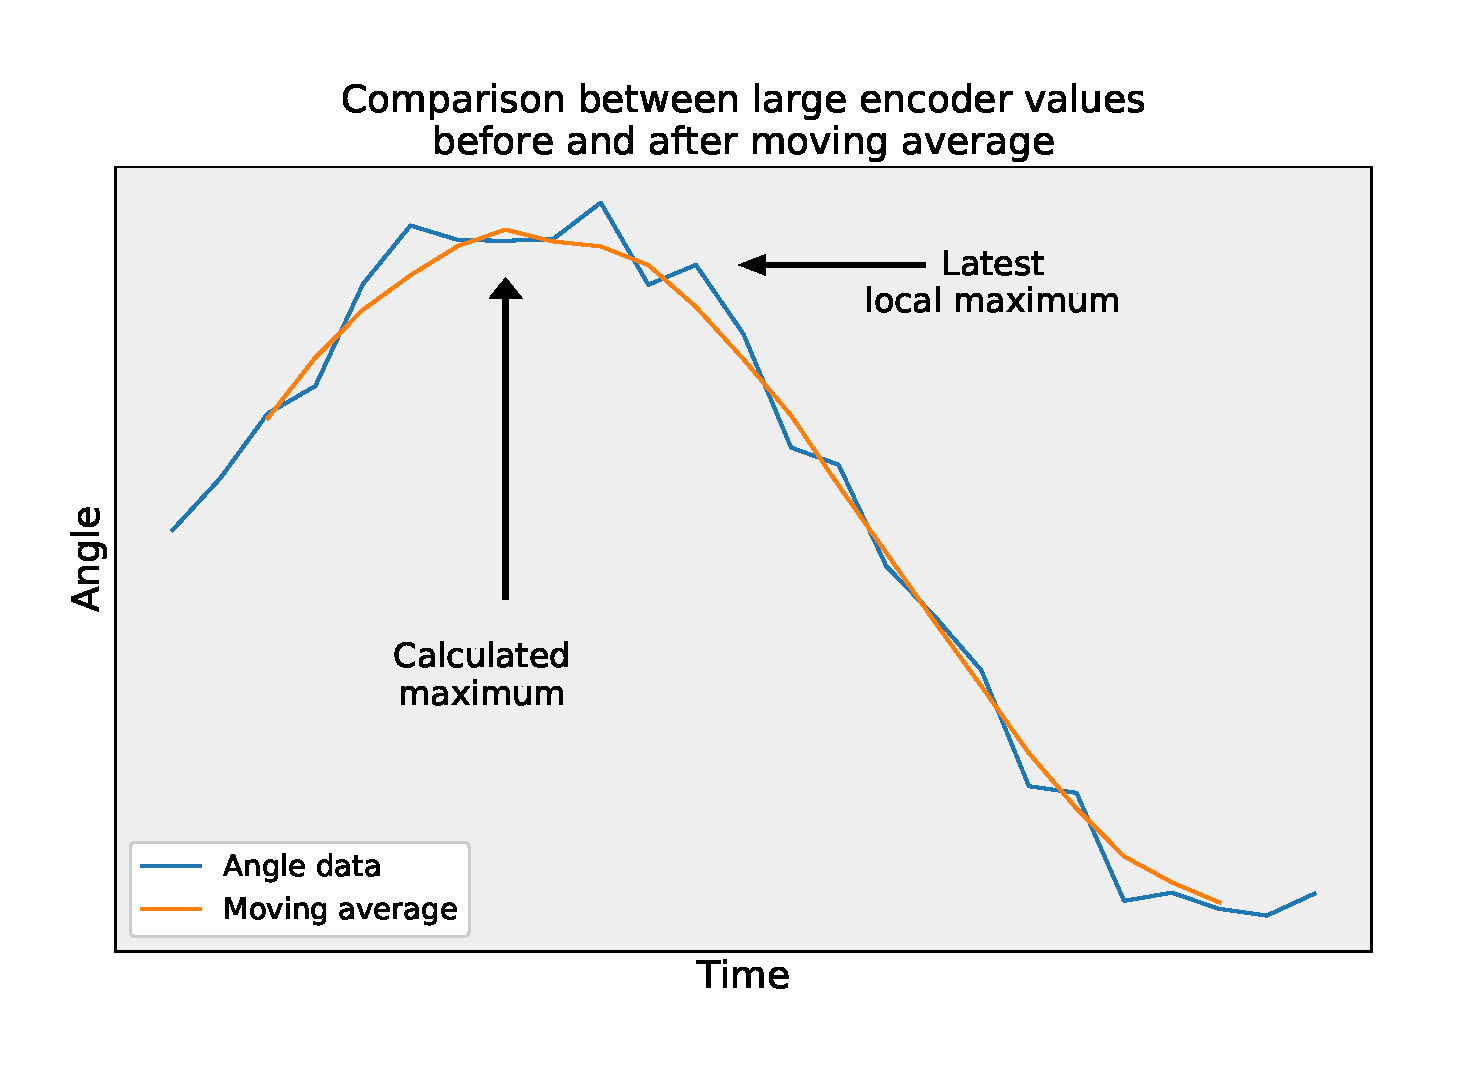
\includegraphics[width=1.0\textwidth]{MovingAverageDiagram.eps}}
    \end{figure}


This process is repeated every half period, whenever Nao crosses the centre point, such that the next maxima time can be calculated before it is reached. From here the only decision that needs to be made is whether it is better to swing before the maxima, at the maxima, or after the maxima for the greatest amplitude swing. An advantage of this algorithm is that the estimate of the period is constantly updated, such that the calculation of the maxima time remains accurate for all amplitudes (as long as there is sufficient build up time to calculate the previous period).

TODO: Advantages and disadvantages of this method
Advantages: Can predict much before the peak allowing offset to decide when is best  
Disadvantages: Only works for small amplitude increases at a time, linear interpolation only works for fast sample speed, smoothing won't remove all local maxima

\subsection{Increasing and Decreasing Amplitude}


\subsubsection{Parametric Pumping}
Jon: Talk about two extra positions defined for this motion, the idea behind the algorithm, results try to fit to exponential curve to see if it multiplies amplitude by fixed fraction like worksheet showed, any limitations, were two positions just different in vertical centre of mass or did horizontal distance change too

\subsubsection{Torque Method TODO: BETTER NAME FOR THIS}
David: Say used previous defined positions, different methods for each algorithm (quarter period, integreation of theory team calculation of max angle), results for each, try to fit maximum amplitude peaks to linear to see if proportional to distance rocked or not, how results varied on different parameters such as if he swings before peak, during, or after, limitations to each method.
Calculations of offset parameters to maximise amplitude gain and comparison of each plot

\subsection{Maintaining Amplitude}
Chenglong: different subsubsection for each method you used, first outline the idea behind each algorithm, then show the results for each, compare and contrast after you have shown results for each, which was easiest to code, had the finest control over the angle (calculate variance on the maximum amplitude of the swing), which is most efficient, anything else you decide is good

\subsection{Chaining together algorithms}
\textit{If i get old joe working I'll write about it briefly here - james}


\subsubsection{Conclusion}
Everyone: Think this should just be how to improve, any difficulties of the setup, which is the best method and why etc

\section{Triple Pendulum}

    \begin{figure}[!htb]
        \centering
        \captionbox
             {Angleplot.\label{angleplot}}
             {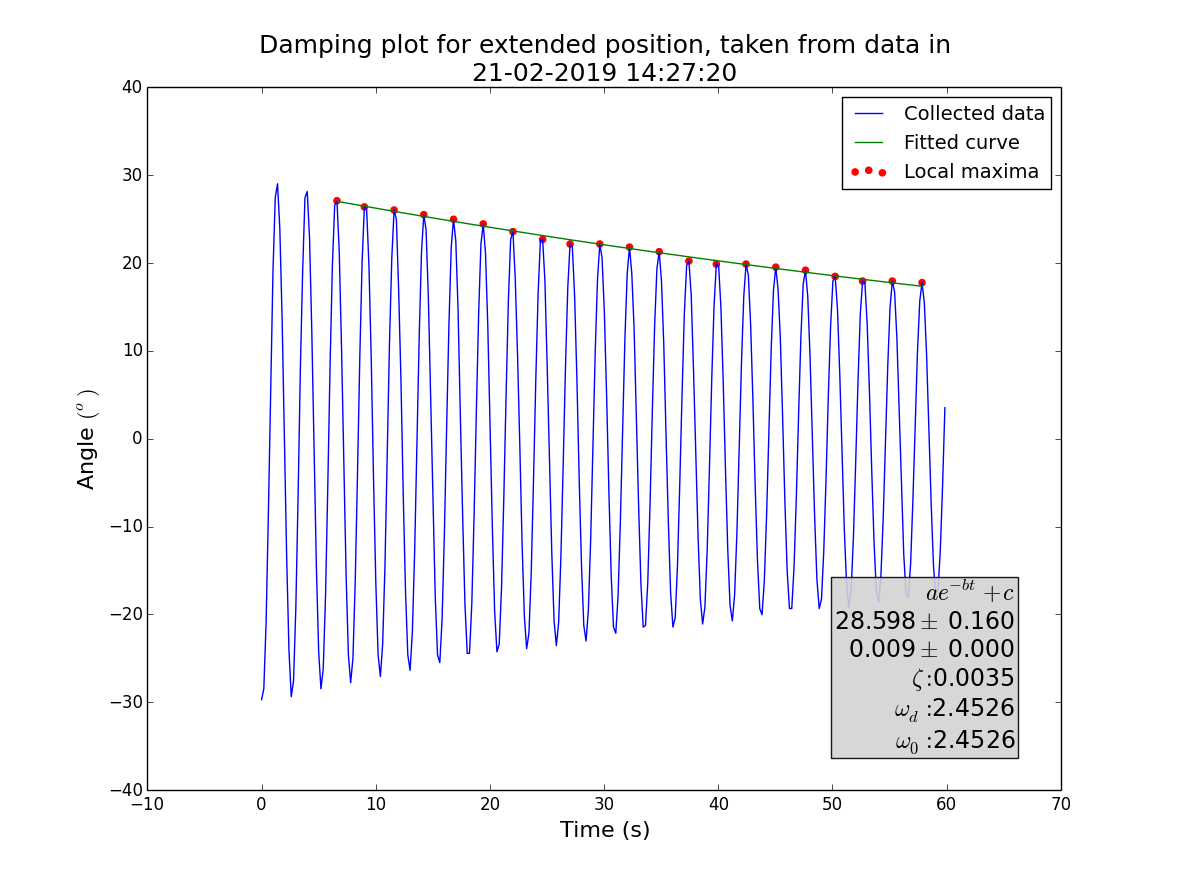
\includegraphics[width=1.0\textwidth]{ExtendedPositionDamping.png}}
    \end{figure}

\subsection{Start Up}
\textit{We will probably just copy the code straight over so just say that.}


\appendix
\section{Appendix}
\subsection{Wiki} \label{sec:wiki}
\ruleline{George Sheppard}
Throughout this project, there were a large amount of issues found when trying to connect to: NAO, Webots, and the hinge encoders etc. For this reason a wiki was created to document how to set everything up correctly. This wiki is available at: https://github.com/GeorgeSheppard/Robotics. Alongside this wiki is the final code, including how to use it, the report, and any analysis files used to create plots. Feel free to clone this repository and add to it such that there remains a comprehensive guide for each year.

\subsection{Webots}
\ruleline{James Doering}
Webots offers a substantial amount of uses - throughout this project Webots was used to test the interface and algorithms away from the lab, and to find accurate estimates for NAO's centre of mass in different positions. However, Webots did not offer much in useful physical simulations - the simulated swing would often fail, and physics would quickly go out of sync if the target frame-rate was missed momentarily. In order to interface with Webots from the NAOQI python library (supplied by Aldebaran/SoftBanks), the NAOQISIM controller was required - this acted as a 'virtual robot' to translate from Python script written with NAOQI to the NAOQISIM controller in Webots, which controlled the simulated NAO. This proved difficult to achieve, only being possible with certain software configurations. It is highly recommended that this is done on a linux operating system, otherwise there will be errors between 32 and 64 bit versions of python and NAOQI/NAOQISIM. The version of NAOQI required to connect to Webots is different to the version required to connect to the real NAO - as of writing, Webots/NAOQISIM requires NAOQI 2.1.4.13, whereas NAO requires NAOQI 1.14.5. Further explanation can be seen on the wiki decribed in section \ref{sec:wiki}.

\bibliographystyle{ieeetr}
\bibliography{References}
\end{document}